\documentclass{article}

\usepackage{amsmath}
\usepackage{amsfonts} % For math fonts.
\usepackage{amssymb} % For other math symbols not covered by amsmath.
\usepackage[pdftex]{graphicx} % For pictures, use \includegraphics[scale=decimal]{pic.png}; must be a .png file type.
\usepackage{multicol}
\usepackage{textcomp}
\usepackage[colorlinks = true, urlcolor = blue]{hyperref}
\usepackage{enumitem}
\usepackage{graphbox} 
\usepackage{subfig}
\usepackage{multicol}
\usepackage{nopageno}
\usepackage{bm}


\usepackage{tikz}
\usetikzlibrary{positioning, calc}
\usetikzlibrary{shapes.geometric,angles,quotes}
\usepackage{tikz-3dplot}


%page formatting
\usepackage{fullpage}
\setlength{\parindent}{0pt}


\newcommand{\tab}{\hspace*{0.25in}}
\newcommand{\csq}[1]{\reflectbox{''}#1''}  %This produces CS style quotes.
\newcommand{\csqt}[1]{\text{\reflectbox{''}#1''}}  %This produces CS style quotes as text.


\usepackage{listings}
\lstset
{ %Formatting for code in appendix
    language=Python,
    basicstyle=\footnotesize,
    numbers=left,
    stepnumber=1,
    showstringspaces=false,
    tabsize=2,
    breaklines=true,
    breakatwhitespace=false,
}


\begin{document}



%split_point

%\end{document}
Lone Star \hfill Loops quiz\\
section 4\\
\begin{enumerate}
\item (4.1)  
		%https://edabit.com/challenge/aqDGJxTYCx7XWyPKc
		Write a program that asks the user for an integer.  Calculate (and then print) the 
		sum of all square numbers up to and including the user's number.

		For example, 
		\begin{itemize}
			\item if user\_number = 3, the result should be 14 since $1^2 + 2^2 + 3^2 = 14$.
			\item if user\_number = 8, the result should be $1^2+2^2+3^2+4^2+5^2+6^2+7^2+8^2=204$.
		\end{itemize}

%end_of_questions

\item (4.2)  
		%https://edabit.com/challenge/ksZrMdraPqHjvbaE6
		Write a program that repeatedly asks the user for integers until a negative integer is 
		given.\\  Report back the largest \textbf{even} number the user entered 
		(not including the negative number).  \\
		If the user didn't enter any even numbers report back $-1$.

		For example, \\ \ \hfill
		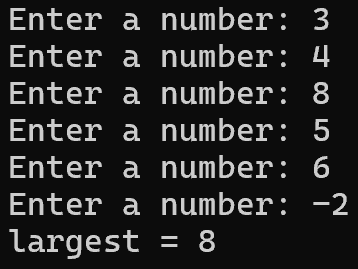
\includegraphics[height = 1.2in]{./imgs/largestEven1.PNG} \hfill  
		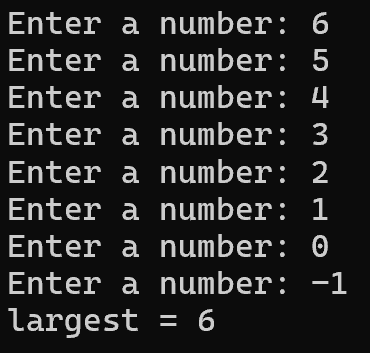
\includegraphics[height = 1.5in]{./imgs/largestEven2.PNG} \hfill  
		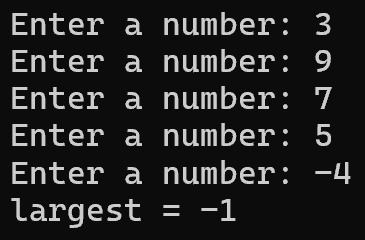
\includegraphics[height = 1.2in]{./imgs/largestEven3.PNG} \hfill \

%end_of_questions

\item (4.3)  
		%https://edabit.com/challenge/xR248CxGSsSrNK5Za
		You are the newest rug fashion designer on the scene, but you're running out of ideas. 
		Write a program that will help you design rugs.  The program should ask for a width, 
		a length, and pattern, and then create a rug consisting of that pattern and dimensions.

		For example, \\ \ \hfill
		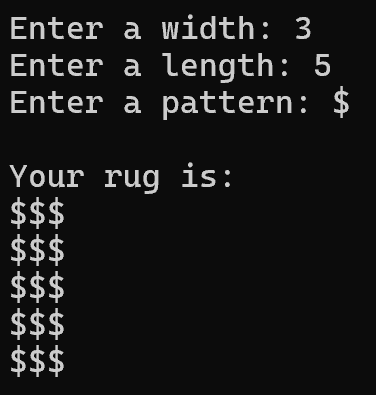
\includegraphics[width = 1.5in]{./imgs/rug1.PNG} \hfill  
		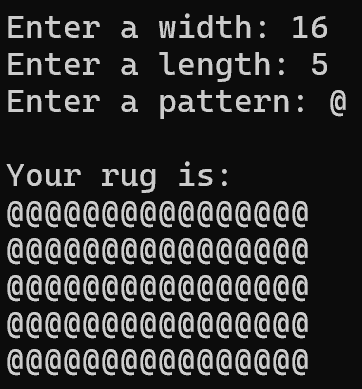
\includegraphics[width = 1.5in]{./imgs/rug2.PNG} \hfill \


\end{enumerate}
\pagebreak
Dot Matrix \hfill Loops quiz\\
section 5\\
\begin{enumerate}
\item (4.1)  
		Using a loop, write code to calculate the sum of all odd numbers between 50 and 517. 
		Print the result.


\item (4.2)  
		%https://edabit.com/challenge/ksZrMdraPqHjvbaE6
		Write a program that repeatedly asks the user for integers until a negative integer is 
		given.\\  Report back the largest \textbf{even} number the user entered 
		(not including the negative number).  \\
		If the user didn't enter any even numbers report back $-1$.

		For example, \\ \ \hfill
		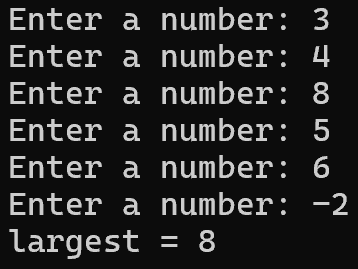
\includegraphics[height = 1.2in]{./imgs/largestEven1.PNG} \hfill  
		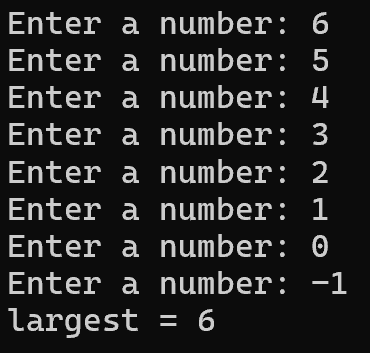
\includegraphics[height = 1.5in]{./imgs/largestEven2.PNG} \hfill  
		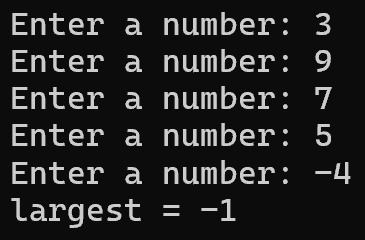
\includegraphics[height = 1.2in]{./imgs/largestEven3.PNG} \hfill \

%end_of_questions

\item (4.3)  
		Ask the user for an integer height, and then build a triangle of asterisks (*) 
		with that height.

		For example, \\ \ \hfill
		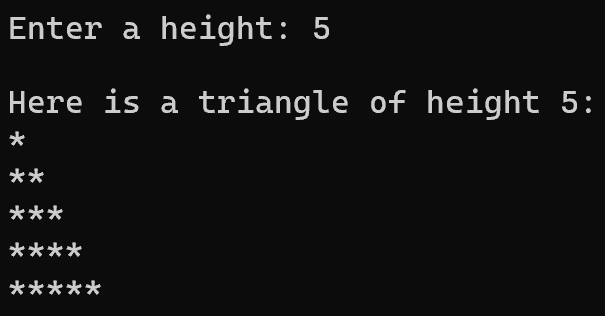
\includegraphics[height = 1.2in]{./imgs/triangle1.PNG} \hfill  
		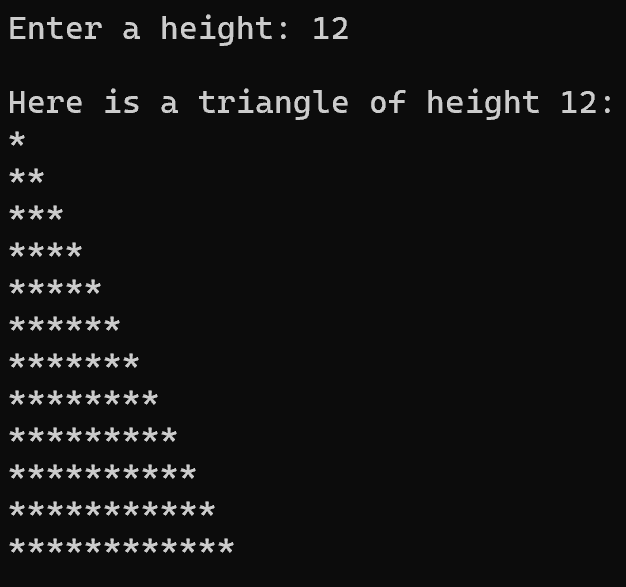
\includegraphics[height = 1.4in]{./imgs/triangle2.PNG} \hfill  \

%end_of_questions

\end{enumerate}
\pagebreak
Dark Helmet \hfill Loops quiz\\
section 4\\
\begin{enumerate}
\item (4.1)  
		%https://edabit.com/challenge/6Pf5GGG6HnzbB95gf
		Write code that asks the user for an integer and then prints each number that is a 
		factor of the input.
	
		For example, \\ \ \hfill
		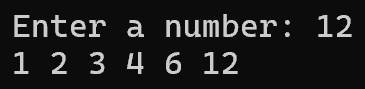
\includegraphics[height = .35in]{./imgs/factors1.PNG} \hfill  
		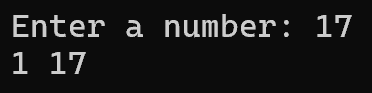
\includegraphics[height = .35in]{./imgs/factors2.PNG} \hfill  
		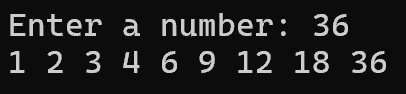
\includegraphics[height = .35in]{./imgs/factors3.PNG} \hfill \


\item (4.2)  
		Write a program that repeatedly asks the user for integers until a negative integer is 
		given. \\ The program should keep track of the sum of the numbers and print the sum at the 
		end \\(not including the negative number).

		For example, \\ \ \hfill
		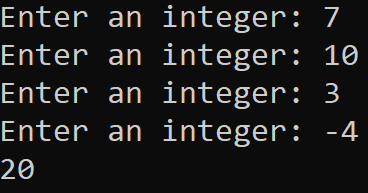
\includegraphics[width = 2.in]{./imgs/AddCalc2.PNG} \hfill  
		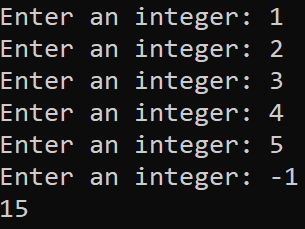
\includegraphics[width = 2.in]{./imgs/AddCalc1.PNG} \hfill \


\item (4.3)  
		%https://edabit.com/challenge/xR248CxGSsSrNK5Za
		You are the newest rug fashion designer on the scene, but you're running out of ideas. 
		Write a program that will help you design rugs.  The program should ask for a width, 
		a length, and pattern, and then create a rug consisting of that pattern and dimensions.

		For example, \\ \ \hfill
		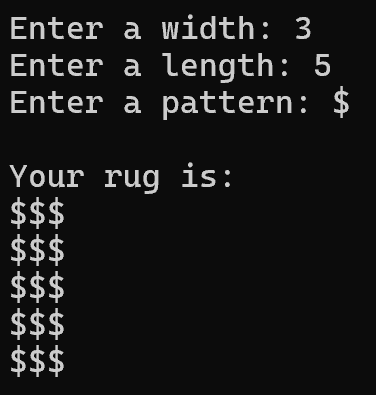
\includegraphics[width = 1.5in]{./imgs/rug1.PNG} \hfill  
		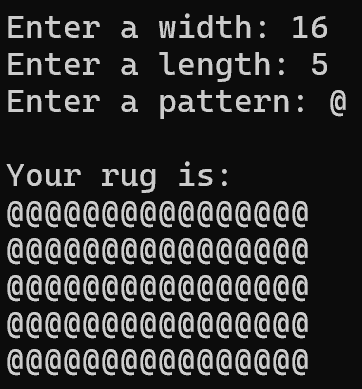
\includegraphics[width = 1.5in]{./imgs/rug2.PNG} \hfill \


\end{enumerate}
\pagebreak
President Skroob \hfill Loops quiz\\
section 1\\
\begin{enumerate}
\item (4.1)  
		Write a program that asks the user for a word and then, \underline{using a loop}, 
		prints every other letter of the word starting with the second letter.

		Examples:
		\begin{itemize}
			\item if user\_word = \csq{counterattack}, the result should be \csq{oneatc}
			\item if user\_word = \csq{banana sunday}, the result should be \csq{aaasna}
		\end{itemize}


\item (4.2)  
		Given a positive integer $n$, the following rules will always create a sequence that 
		ends with 1, called Hailstone Sequence:
		\begin{enumerate}
			\item If $n$ is even, divide by 2
			\item If $n$ is odd, multiply by 3 and add 1 (i.e. $3n+1$)
			\item Continue until $n$ is 1
		\end{enumerate}
		Write a program that prints the hailstone sequence starting at $n=25$.


\item (4.3)  
		Ask the user for an integer height, and then build a triangle of asterisks (*) 
		with that height.

		For example, \\ \ \hfill
		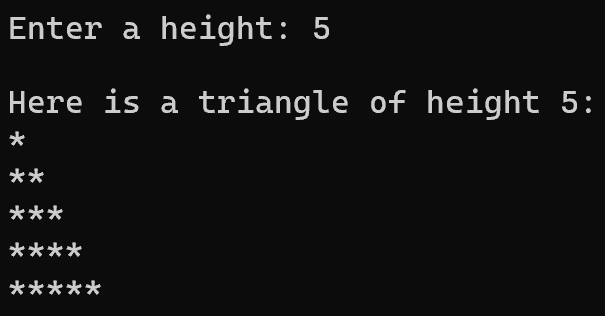
\includegraphics[height = 1.2in]{./imgs/triangle1.PNG} \hfill  
		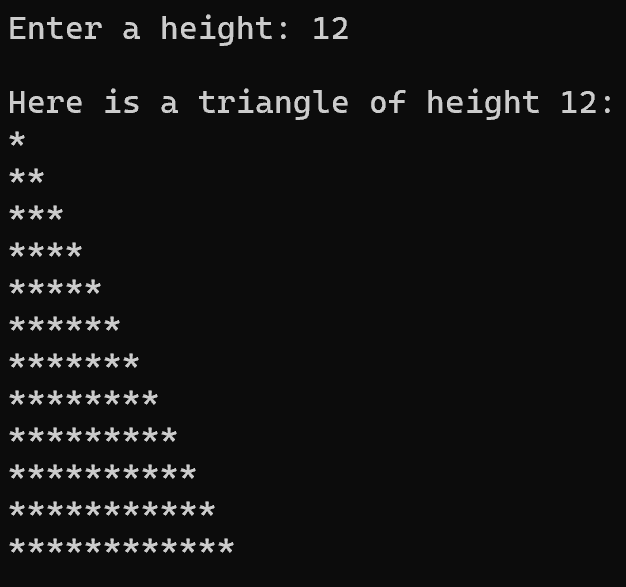
\includegraphics[height = 1.4in]{./imgs/triangle2.PNG} \hfill  \

%end_of_questions

\end{enumerate}
\pagebreak
\end{document}